\documentclass[10pt,twocolumn,letterpaper]{article}

\usepackage{cvpr}
\usepackage{times}
\usepackage{epsfig}
\usepackage{graphicx}
\usepackage{amsmath}
\usepackage{amssymb}
\usepackage{caption}
\usepackage{subcaption}

% Include other packages here, before hyperref.

% If you comment hyperref and then uncomment it, you should delete
% egpaper.aux before re-running latex.  (Or just hit 'q' on the first latex
% run, let it finish, and you should be clear).
\usepackage[breaklinks=true,bookmarks=false]{hyperref}

\cvprfinalcopy % *** Uncomment this line for the final submission

\def\cvprPaperID{****} % *** Enter the CVPR Paper ID here
\def\httilde{\mbox{\tt\raisebox{-.5ex}{\symbol{126}}}}

% Pages are numbered in submission mode, and unnumbered in camera-ready
%\ifcvprfinal\pagestyle{empty}\fi
%\setcounter{page}{4321}
\begin{document}

%%%%%%%%% TITLE
\title{Cameras Simulating Lidar through CNN}

\author{Zhenghao Fei\\
BAE, UC, Davis\\
{\tt\small zfei@ucdavis.edu}
% For a paper whose authors are all at the same institution,
% omit the following lines up until the closing ``}''.
% Additional authors and addresses can be added with ``\and'',
% just like the second author.
% To save space, use either the email address or home page, not both
\and
Chen Peng\\
MAE, UC, Davis\\
{\tt\small penchen@ucdavis.edu}
\and
Shubo Chen\\
ECE, UC, Davis\\
{\tt\small sbochen@ucdavis.edu}
}
\maketitle
%\thispagestyle{empty}

%%%%%%%%% ABSTRACT
\begin{abstract}
Depth information are crucial in areas such as obstacle avoidance, autonomous mapping, route planning and navigation. Among various depth sensors that are currently available in the market, Lidars are popularly used in measuring depth information to surrounding environment because of its accuracy, precision and flexibility. However, Lidars can be very costly. In this project, we attempted to use convolutional neural network to train a two-eye camera with depth information detected from a 2D Lidar to see if the camera would learn how to extract depth information from images it captures so it could be a potential substitution of the expensive lidar. As in our knowledge, we are the first attempt that uses two images of a two-eye camera(generates two images at a time) as input to train a network to simulate lidar behavior so far. 
\end{abstract}

%%%%%%%%% BODY TEXT
\section{Introduction}

Depth information are crucial in areas such as obstacle avoidance, autonomous mapping, route planning and navigation. Among various depth sensors that are currently available in the market, Lidars are popularly used in measuring depth information to surrounding environment because of its accuracy, precision and flexibility. However, Lidars can be very costly. As from the papers we read\cite{kyto2011method},\cite{jones2011head}, \cite{diebel2004simultaneous} we learned that stereo cameras are able to detect depth information and they are relatively cheap compared to most of depth sensors, but previous methods like triangulation are not very effective in terms of accuracy and computational cost. Therefore, we propose this approach that trains a deep neural network on two cameras to obtain accurate depth values from targeted area just like what the precise sensors do. For this project, we run a ZED two-eye camera and an 2D lidar on a robotic system simultaneously in order to obtain images and lidar measured points. Then we use measured depth as ground truth, images as inputs to train a deep neutral network so that the images can be transformed to lidar points. We used ROS(Robotic Operating System) to monitor and control the camera and lidar and all the data were manually collected and stored by the team. 34K data were used as training data which was fed into the network and 1.5K data were used to perform validation. The network was constructed and operated in Tensorflow. The idea from this project may be extended to use some latent information obtained from sensor A to learn obvious and useful information from sensor B. Images contain much of such latent features of objects which can be extracted by DNN, just like human eyes do.
%-------------------------------------------------------------------------
\section{Related work}
Our work mainly focused on how to design neural network to extract useful visual representations of depth information from two images and calculate the regression value of  2-D depth in front of the robots.
\subsection{Traditional methods to calculate depth from two images}
Paper \cite{saxena2007depth} used images from two cameras to triangulate and estimate distances relative to a robot. Monocular visual cues were used in the images to perform the estimation. They suggested that depth information indeed hide in two stereo camera pictures. Therefore, we can theoretically estimate the depth information from a two-eye stereo camera.  

\subsection{Supervised learning}

In paper \cite{pinto2016curious}, the author designed a Siamese neural network to predict pushing angle and force exerting point on an object by inputting two images-Object before pushing and after pushing. Here they used 4 layers CNN and two fully connected network to predict 6 output of regression values. In addition, they also used a one row CNN to calculate the  predicted regression value of material hardness features of objects (slope and intercept of supporting force line). In this paper, the author mainly used the updated weights to perform image recognition, but did not testify the accuracy of their regression prediction. Paper used NYU Depth v2 [indoor] dataset to train a DNN to extract an accurate dense 3D interpretation based on one single image. They showed the result of dense information extracted from images but the labels were obtained from Microsoft Kinect stereo camera, whose depth information was calculated from classic methods and not as accurate as 2-D lidar. In our approach, we uses labels obtained by Lidar directly and expect to achieve better results. 
\section{Approach}
\subsection{Robot platform}
To construct our own datasets, we installed a Zed camera and 2D Lidar on a small robot vehicle. The robot can be controlled to move in a complex depth changing environment. While robot was moving, we recorded the input data-images captured by Zed camera and training labels-2-D Lidar depth information.
\subsubsection{Cameras}
The camera we used is called Zed camera, which is capable of capturing 10 pictures in about one second. \textbf{We only collect images captured in the front.} The size of images taken by the camera is 376*672*3. Since the lidar we use is in 2-D, we sliced the images vertically into three pieces and only kept the middle piece. Therefore, The size became 128*672*3 as raw image inputs. The Zed camera is shown in Figure\ref{zed_camera}
\begin{figure}[t]
	\begin{center}
		%\fbox{\rule{0pt}{2in} \rule{0.9\linewidth}{0pt}}
		\includegraphics[width=0.8\linewidth]{pictures/zedcamera.png}
	\end{center}
	\caption{Zed Cameras}
	\label{zed_camera}
\end{figure}


\subsubsection{Lidar}
We used RPLIDAR, a 2D lidar to sense the depth information at its sensing height. 2-D Lidar can sense the depth information in 360 degrees of its surrounding environment.The lidar is shown in Figure \ref{lidar} and the sensing process is visualized in Figure\ref{lidar_sensing}.

\begin{figure}
	\centering
		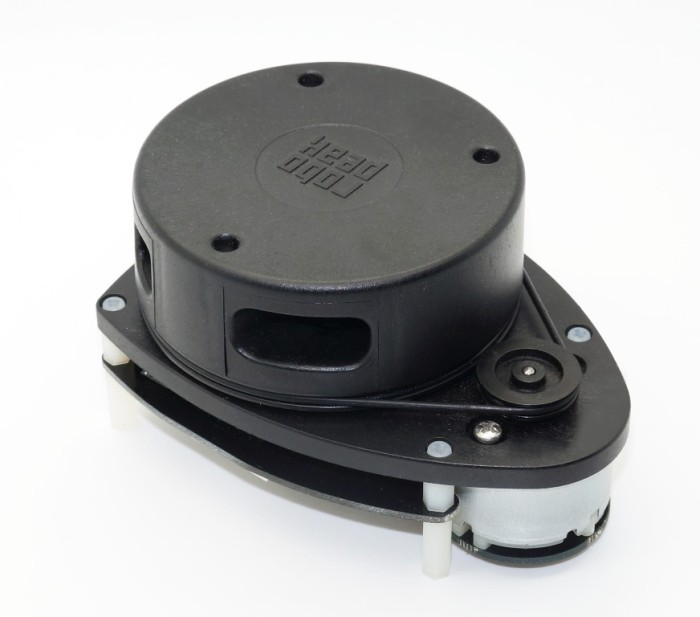
\includegraphics[width=.3\linewidth]{pictures/lidar.jpg}
		\caption{RPLIDAR 2D lidar}
		\label{lidar}

\end{figure}
\begin{figure}
		\centering
		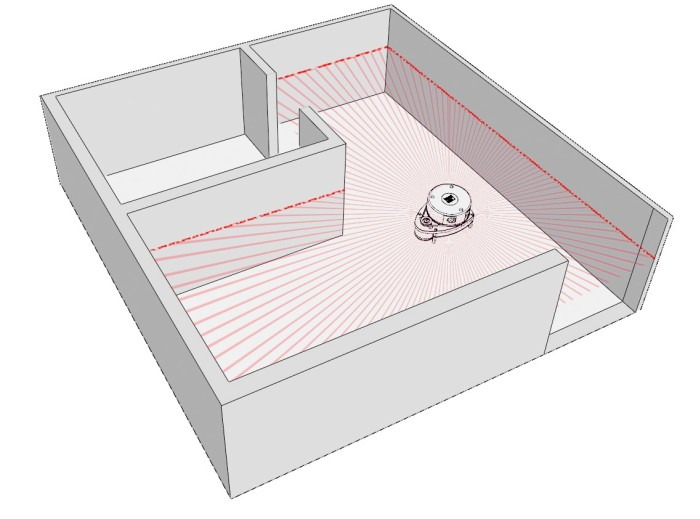
\includegraphics[width=.8\linewidth]{pictures/lidar_sensing.jpg}
		\caption{Lidar sensing the environment}
		\label{lidar_sensing}
\end{figure}

As the span view of the zed camera is 120 degrees, therefore we selected only depth information in 120 degrees in front of the lidar as labels. 
%Mermin's description of how to write mathematics:
%\url{http://www.pamitc.org/documents/mermin.pdf}.
\subsubsection{ROS}
In order to collect the inputs and labels simultaneously, we ran them on the Robot Operating System (ROS) to pack them in the series of recorded time. ROS is a flexible framework for writing robot software. It is a collection of tools, libraries, and conventions that aims to simplify the task of creating complex and robust robot behavior across a wide variety of robotic platforms\cite{ROSabout}. We constructed a ROS node for lidar to publish the labels and another node for zed camera to publish inputs. At the same time, we constructed a subscriber to record all the data and pack them into ROS bags. After data collection, we ran ‘rosbag play’ to publish all the inputs and labels in time series. Meanwhile, we subscribed the publishing and keep the record of all data. At last, we matched all the inputs and corresponding labels based on recorded time.  Figure \ref{two_images} shows the two sliced images captured by camera, and Figure \ref{lidar_visual} is an illustration of depth information sensed by Lidar. The red area is the 120-degree ranging we selected as labels.
\begin{figure}[t]
\begin{center}
%\fbox{\rule{0pt}{2in} \rule{0.9\linewidth}{0pt}}
\includegraphics[width=0.8\linewidth]{pictures/two_images.png}
\end{center}
   \caption{Two images captured by camera}
\label{two_images}
\end{figure}

\begin{figure}[t]
	\begin{center}
		\includegraphics[width=0.8\linewidth]{pictures/lidar_visual.png}
	\end{center}
	\caption{Lidar data}
	\label{lidar_visual}
\end{figure}

\section{Network Architecture}
The network architecture is showed in Figure \ref{network} below. We tuned the size of images and convolutional filters during our experiments but keep the main structure the same.

\begin{figure}
\centering
   \includegraphics[width=8cm]{pictures/network_architecture.png}
   \caption{CNN architecture}
\label{network}
\end{figure}

\textbf{Two stream inputs:} Our task needs information from both left and right images thus we built two input streams to process two inputs. Unlike Siamese network, the upper stream and lower stream don’t share weights. In this way the convolutional neural network treat two images differently which make more sense since two images has different viewpoints. 


\textbf{Extract edges, features, objects and scenes:} The convolutional layers are used for edge and feature extraction, as it may help the network to predict the depth more precisely. If we use a deeper convolutional network architecture, higher level notion of object and scene can also be used by the network. We believe that with the help of edge, feature, object and scene notion, we can extract more depth information from images than the traditional way.


textbf{Regression:} The fully connected layers are used for nonlinear regression, we hope the network can figure out the tradition way of triangulate and estimate distances. Different from many applications of using convolutional neural work to do classification, our network is doing regression job. It seems harder than classification, but we would like to get more accurate gradient information from RMSE loss function rather than use a cross-entropy loss.


At this stage, we choose a relatively simple architecture to verify our idea, so it is easier to train and needs less amount of data to overcome overfitting. We can increase the depth when we have more data. 


Training details:Our convolutional neural network is implemented in Tensorflow  with a GTX 960 GPU. The training dataset has 34K examples and the validation set has 1.5K. We use Gradient Descent Optimizer with learning rate decay factor 0.1 every 10000 epochs. 

\section{Results}
We defined our loss function as root mean square error of 120 points of distance.
\begin{equation*}
rmse =\frac{\sqrt{\sum\limits_{i=1}^{120} (y_i-y_i')^2}}{120}
\end{equation*}

\begin{figure}
	\begin{subfigure}{.25\textwidth}
		\centering
		\includegraphics[width=1\linewidth]{pictures/train.png}
		\caption{train epochs vs. train loss}
		\label{loss}
	\end{subfigure}%
	\begin{subfigure}{.25\textwidth}
		\centering
		\includegraphics[width=1\linewidth]{pictures/validate.png}
		\caption{train epochs vs. validation loss}
		\label{rmse}
	\end{subfigure}
	\caption{Loss and rmse}
	\label{result}
\end{figure}

\begin{figure}
	\begin{subfigure}{.25\textwidth}
		\centering
		\includegraphics[width=1\linewidth]{pictures/pair1-1.png}
		\label{label1}
	\end{subfigure}%
	\begin{subfigure}{.25\textwidth}
		\centering
		\includegraphics[width=1\linewidth]{pictures/pair1-2.png}
		\label{result1}
	\end{subfigure}
	\begin{subfigure}{.25\textwidth}
		\centering
		\includegraphics[width=1\linewidth]{pictures/pair2-2.png}
		\label{label2}
	\end{subfigure}%
	\begin{subfigure}{.25\textwidth}
		\centering
		\includegraphics[width=1\linewidth]{pictures/pair2-1.png}
		\label{result2}
	\end{subfigure}
	\begin{subfigure}{.25\textwidth}
		\centering
		\includegraphics[width=1\linewidth]{pictures/pair4-2.png}
		\caption{Labels}
		\label{label3}
	\end{subfigure}%
	\begin{subfigure}{.25\textwidth}
		\centering
		\includegraphics[width=1\linewidth]{pictures/pair4-1.png}
		\caption{Results}
		\label{result3}
	\end{subfigure}
	\caption{Succeed cases}
	\label{good results}
\end{figure}

\begin{figure}
\begin{subfigure}{.25\textwidth}
	\centering
	\includegraphics[width=1\linewidth]{pictures/bad.png}
	\caption{Labels}
	\label{label4}
\end{subfigure}%
\begin{subfigure}{.25\textwidth}
	\centering
	\includegraphics[width=1\linewidth]{pictures/bad(1).png}
	\caption{Results}
	\label{result4}
\end{subfigure}
	\caption{Failed cases}
	\label{bad results}
\end{figure}



The unit is in meter. It can be considered as average error for every point. 
\subsection{Train:}
As we can see in Figure \ref{result} as number of training epochs increase, the loss reduces to a very low number, it even approaches to 0 after enough time of training, which indicates our convolutional neural network has enough capacity to learn.

\subsection{Validation:}
However, for the validation loss, we can see it goes down to about 1.8m RMSE then start to increase, which indicates that the model starts overfitting. Due to time constraint we only collected 34K training data, we suspect that the small size of data causes this overfitting problem. Our former experiment with 5K training data produces even worse RMSE which is 2.8m. We believe that more data would help us get lower RMSE and some data augmentation and overfitting preventing methods can also help in this case. Figure \ref{good results} are some of the cases that we think can used to represent succeed ones. We can tell that the result and label have the same pattern but in other cases as shown in Figure \ref{bad results}, the result failed to predict the depth from the image.


\section{Conclusion}
In this project we trained a neural network to learn how to extract depth information from images in order to determine if a cheap stereo camera can simulate the functionality of an 2D Lidar. With the experiments and results, we demonstrated that as more training data was fed in the network, the loss was decreasing, showing that the network is learning depth information from the given inputs and labels. However, from the figure of rmse of validation dataset, it is obvious that after the best score (1.79m), the model started overfitting. Possible explanations are that our training dataset is not large enough or the network is too complex. 

\section{Future Work}

In future work, we will first look at the issue of overfitting. Possible solutions are enlarge our training dataset and borrow other pre-trained CNNs and fine tune their architecture to fit our goal. Meanwhile, we will find a way to visualize the weights and outputs to see what we have learned to help us have a better understanding of the process. 

{\small
\bibliographystyle{ieee}
\bibliography{egbib}
}

\end{document}
